%%%%%%%%%%%%%%%%%%%%%%%%%%%%%%%%%%%%%%%%%%%%%%%%%%%%%%%%%%%%%%%%%
% Tese de Doutorado / Dept Fisica, CFM, UFSC                    %
% Andre@UFSC - 2014                                             %
%%%%%%%%%%%%%%%%%%%%%%%%%%%%%%%%%%%%%%%%%%%%%%%%%%%%%%%%%%%%%%%%%

%:::::::::::::::::::::::::::::::::::::::::::::::::::::::::::::::%
%                                                               %
%                          Capítulo 6                           %
%                                                               %
%:::::::::::::::::::::::::::::::::::::::::::::::::::::::::::::::%

%***************************************************************%
%                                                               %
%         Testes da decomposição morfológica espectral          %
%                                                               %
%***************************************************************%

\chapter{Testes da decomposição morfológica espectral}
\label{sec:test}

A decomposição morfológica espectral, aplicada ao cubo de dados de uma galáxia,
resulta numa sequência de modelos morfológicos em função do comprimento de onda.
Avaliando os modelos como imagens, é possível montar cubos de dados espectrais
para as componentes do modelo. Ou seja, com um modelo bojo e disco, a
decomposição de um cubo de dados de uma galáxia gera dois cubos, um para o bojo
e outro para o disco.

De posse destes cubos de dados espectrais das duas componentes, pode-se começar
a ponderar o significado de um de seus {\em spaxels}. Intuitivamente, espera-se
que, espectroscopicamente, ele se pareça a um {\em spaxel} da galáxia original.
No entanto, nada garante que ele deva ser parecido com espectro algum, afinal o
cubo espectral da componente morfológica é resultado de um processo
computacional bastante complexo, que leva em conta apenas informações espaciais.
Também, como se comentou na Seção \ref{sec:morph:comp:bd}, é preciso ter cuidado
ao interpretar o resultado de um ajuste de modelo empírico. Isto é ainda mais
importante em casos onde se faz este ajuste de forma automatizada, sem
inspecionar cada imagem e seus modelos de forma individual, como é o caso da
decomposição morfológica espectral.

O próximo Capítulo descreve em detalhes a decomposição morfológica espectral de
cubos de dados do CALIFA. A fim de determinar se o método funciona, neste
capítulo foi construído um modelo de galáxia simples, com parâmetros
morfológicos e espectros das componentes conhecidos. A decomposição foi aplicada
a esta galáxia sintética, com o resultado apresentado a seguir.

%***************************************************************%
%                                                               %
%                   Construindo uma galáxia                     %
%                                                               %
%***************************************************************%
\section{Construindo uma galáxia}

Não é objetivo deste exercício modelar uma galáxia realista. Os parâmetros foram
escolhidos apenas para que o modelo que se assemelhe a uma galáxia real, sem
qualquer necessidade de ser fisicamente possível tal galáxia existir. O modelo
utilizado foi um bojo com uma lei de de Vaucouleurs (Sérsic com $n=4$) e um
disco com uma lei exponencial (ver Seção \ref{sec:morph:comp:bd}), cada
componente com um perfil elipsoidal distinto dado por uma elipticidade
($\epsilon = 1 - b/a$, onde $a$ e $b$ são os semieixos maior e menor) e um
ângulo de posição (P.A.) medido em sentido anti-horário a partir do eixo
horizontal. Os parâmetros do modelo original não listados na Tabela
\ref{tab:testeModeloOriginal}.

\begin{table}
\begin{tabular}{ l  c | l  c }
  \hline
  \multicolumn{4}{c}{\textbf{Modelo original}} \\
  \multicolumn{2}{c}{\textbf{Bojo}} & \multicolumn{2}{c}{\textbf{Disco}} \\
  \hline
  $I_e$ & $2,0$ & $I_0$ & $1.0$ \\
  $r_e$ & $5,0\,\arcs$ & $h$ & $15.0\,\arcs$ \\
  $n$ & $4$ & & \\
  $\mathrm{P.A.}$ & $60^\circ$ & $\mathrm{P.A.}$ & $45^\circ$ \\
  $\epsilon$ & $0,1$ & $\epsilon$ & $0,1$ \\
  \hline
\end{tabular}
\caption[Modelo morfológico original da galáxia sintética]
{Parâmetros do modelo morfológico original da galáxia sintética.}
\label{tab:testeModeloOriginal}
\end{table}

\begin{figure}
	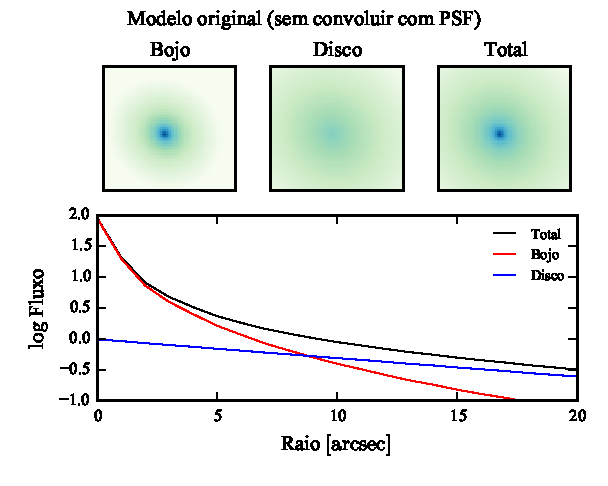
\includegraphics{figuras/simulation_initmodel}
	\caption[Modelo morfológico inicial da galáxia sintética]
	{Modelo morfológico da galáxia sintética utilizada para testar a decomposição
	morfológica espectral. A este modelo ainda não foi aplicada a convolução com a
	PSF. Acima, a imagem referente às componentes bojo e disco, e total (bojo +
	disco). Abaixo, o perfil radial de brilho, calculado em isofotas da imagem
	total.}
	\label{fig:testInitmodel}
\end{figure}

Este modelo original, mostrado na Figura \ref{fig:testInitmodel}, descreve o
brilho superficial da galáxia no comprimento de onda de normalização escolhido,
$5635\,\angstrom$.

\begin{figure}
	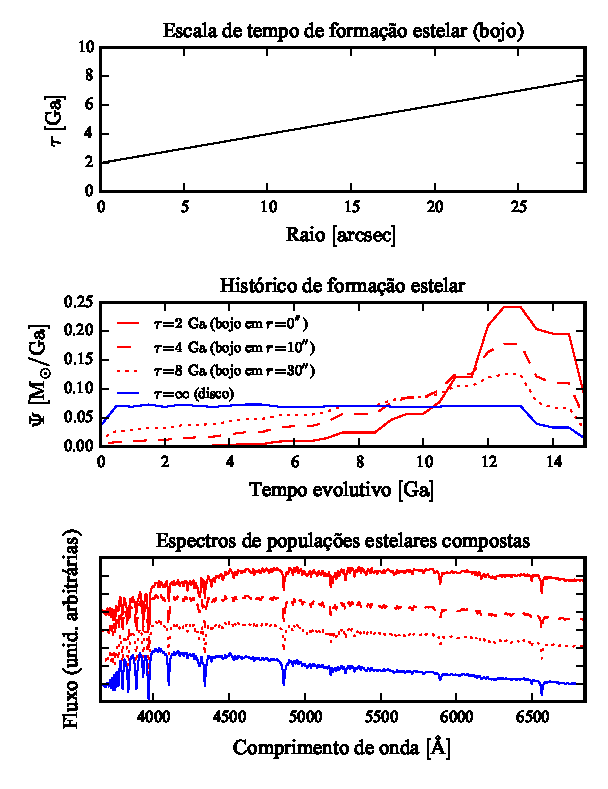
\includegraphics{figuras/simulation_popmodel}
	\caption[Modelos de populações estelares da galáxia sintética]
	{Populações estelares das componentes bojo (em vermelho)
	e disco (em azul) da galáxia sintética. No painel superior, a dependência
	espacial do tempo de escala do decaimento, $\tau$, da SFR do bojo. No painel
	central taxas de formação estelar (SFR), modelados como $\Psi(t) = A \exp
	(-t/\tau)$. A SFR do disco é constante, com $\tau\to\infty$. Abaixo, os
	espectros resultantes, utilizando a base Granada--MILES.}
	\label{fig:testPopmodel}
\end{figure}

Para transformar este modelo num cubo de dados espectral, deve-se estendê-lo na
direção de comprimento de onda. Utilizando espectros de populações estelares
simples (SSP) de uma base e históricos de formação estelar (SFH) sintéticos
para cada componente, obteve-se espectros para cada {\em pixel} da galáxia. Neste
teste, o SFH do disco é sempre o mesmo, independente da posição na componente.
Isto significa que todos os espectros do disco têm a mesma forma, modulados pela
distribuição espacial de brilho dado pelo modelo morfológico (Figura
\ref{fig:testInitmodel}). Já o SFH do bojo varia com a posição, ou seja, os
espectros variam tanto em forma quanto em intensidade. A forma exata dos SFH do
bojo e do disco não é relevante, basta que representem populações
suficientemente diferentes uma da outra. O modelo de populações é mostrado na
Figura \ref{fig:testPopmodel}.

Escolheu-se modelar o SFH do bojo como um surto de decaimento exponencial de
formação estelar com início há $14\,\mathrm{Ga}$, com a taxa de formação estelar
em função do tempo (SFR) dada por $\Psi(t) = A \exp (-t/\tau)$, normalizada de
tal forma que $\int \Psi(t)\,\mathrm{d}t = 1\,\mathrm{M}_\odot$. O SFH do disco
consiste numa SFR constante. A escala de tempo de decaimento $\tau$ tem a sua
dependência espacial, no bojo, dada pela lei linear $\tau = \tau_0 + \alpha r$,
onde $\tau_0$ é o seu valor no núcleo da galáxia e $\alpha$ o seu gradiente.
Foram escolhidos $\tau_0 = 2\,\mathrm{Ga}$ e $\alpha = 0,2\,\mathrm{Ga} /
\arcs$, com um $\tau$ resultante mostrado no o painel superior da Figura
\ref{fig:testPopmodel}. Para o disco, a SFR constante é obtida com
$\tau\to\infty$. Estas SFR sintéticas foram discretizadas para aplicar a uma
base de modelos de SSP. A base utilizada foi a de Granada--MILES, explicada na
Seção \ref{sec:ifs:starlight}. A SFR do bojo e do disco estão mostrados no
painel central da mesma figura, respectivamente em vermelho e azul. A forma das
SFR foge um pouco de uma exponencial devido ao fato de a base de modelos não ser
homogeneamente espaçada em idade. Os espectros finais são obtidos somando os
espectros da base, com o peso dado pelo vetor de população obtido das SFR
sintéticas. O painel inferior da Figura \ref{fig:testPopmodel} mostra os
espectros do bojo para $r = 0$, $10$ e $30\,\arcs$ com o mesmo código de cores
das SFR. O espectro do bojo tem um aspecto de populações velhas no centro da
galáxia ($\tau = 2\,\mathrm{Ga}$), e vai ficando cada vez mais jovem à medida
que se afasta do centro. O espectro do disco é sempre mais jovem do que o do
bojo.

Nenhuma outra propriedade física foi modelada. Adicionar poeira, por exemplo,
modificaria os espectros, mas isto não faria diferença no teste. O importante
aqui é que bojo e disco tenham espectros diferentes, e que os espectros possam
variar de forma com a posição. Por outro lado, a cinemática mereceria um teste
dedicado. Modelar (e levar em conta no ajuste morfológico) o efeito da
cinemática não é uma tarefa trivial, já que bojos e discos têm cinemáticas
completamente distintas. Este é certamente um problema que deve ser visitado no
futuro.

Multiplicando a imagem do modelo pelo conjunto de espectros de cada componente,
obteve-se um cubo de dados espectral para bojo e disco. Para obter o cubo da
galáxia sintética, somaram-se as duas componentes, convoluiu-se com a PSF de
$\mathrm{FWHM} = 2,9\,\arcs$, e adicionou-se ruído gaussiano de $5\%$ (para um
sinal--ruído de $20$). Para deixar o cubo em dimensões parecidas à do CALIFA, os
{\em spaxels} a uma distância $r > 32\,\arcs$ foram mascarados, como aparece nos
painéis superiores da Figura \ref{fig:testFitmodel}, descrita na próxima seção.

%***************************************************************%
%                                                               %
%               Decompondo a galáxia sintética                  %
%                                                               %
%***************************************************************%
\section{Decompondo a galáxia sintética}

O algoritmo da decomposição morfológica espectral é tratado em detalhes no
Capítulo \ref{sec:Decomp}, sendo descrito apenas superficialmente nesta seção.

\begin{figure}
	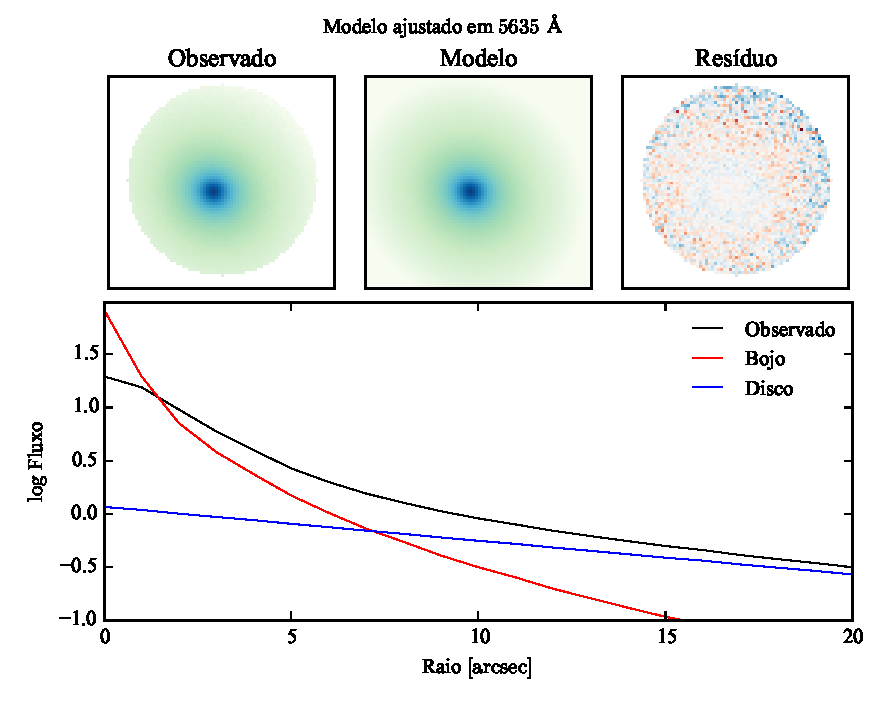
\includegraphics{figuras/simulation_fitmodel}
	\caption[Modelo morfológico inicial do ajuste da galáxia sintética]
	{Modelo morfológico ajustado à galáxia sintética em $5635\,\angstrom$
	utilizando o algoritmo DE. A imagem de resíduo é a diferença entre
	observado e modelo, dividida pelo observado, nos painéis superiores. O perfil
	radial de brilho, no painel inferior, pode ser comparado ao perfil da Figura
	\ref{fig:testInitmodel}. Note que o perfil para o fluxo observado, aqui, está
	convoluído com a PSF.}
	\label{fig:testFitmodel}
\end{figure}

Como o objetivo é fazer a decomposição $\lambda$-a-$\lambda$, o algoritmo
escolhido foi o de L-M (Seção \ref{sec:morph:comp:ajuste}). Ele pode ser
extremamente rápido, mas requer um bom chute inicial. Então, o primeiro passo
na decomposição é encontrar um modelo com valores aproximado das propriedades
das componentes. Para tanto, pode-se utilizar um algoritmo mais complexo, como o
DE, que requer apenas uma faixa de valores para os parâmetros do modelo.
O procedimento de ajuste inicial é descrito em detalhes é descrito na Seção
\ref{sec:Decomp:initmodel}. A decomposição foi feita com a mesma PSF utilizada
para criar o cubo, $\mathrm{FWHM} = 2,9\,\arcs$. Na Seção \ref{sec:test:psf}
discute-se o que acontece quando se utiliza uma PSF diferente da ideal.

A Figura \ref{fig:testFitmodel} mostra o modelo ajustado inicial. O ajuste
foi feito numa faixa de $90\,\angstrom$ ao redor de $5635\,\angstrom$ (a
mesma utilizada para normalizar os espectros antes de rodar o \starlight).
O ajuste foi suficientemente bom, próximo ao modelo original (comparar com a
Figura \ref{fig:testInitmodel}). Os parâmetros do modelo inicial ajustado estão
listados na Tabela \ref{tab:testeModeloInicial}.

\begin{table}
\begin{tabular}{ l c c l c c }
  \hline
  \multicolumn{6}{c}{\textbf{Modelo inicial}} \\
  & \multicolumn{2}{c}{\textbf{Bojo}} & & \multicolumn{2}{c}{\textbf{Disco}} \\
  & \textbf{Ajuste} & \textbf{Original} & & \textbf{Ajuste} & \textbf{Original} \\
  \hline
  $I_e$ & $3,0$ & $2$ & $I_0$ & $1,2$ & $1$ \\
  $r_e$ & $3,9\,\arcs$ & $5\,\arcs$ & $h$ & $14,3\,\arcs$ & $15\,\arcs$\\
  $n$ & $3,4$ & $4$ & & & \\
  $\mathrm{P.A.}$ & $60,3^\circ$ & $60^\circ$ & $\mathrm{P.A.}$ & $46,5^\circ$ &
  $45^\circ$ \\
  $\epsilon$ & $0,1$ & $0,1$ & $\epsilon$ & $0,1$ & $0,1$ \\
  \hline
\end{tabular}
\caption[Modelo inicial ajustado à galáxia sintética]
{Parâmetros do modelo inicial ajustado à galáxia sintética, utilizando o
algoritmo DE.}
\label{tab:testeModeloInicial}
\end{table}


Este ajuste não precisa ser perfeito, ele será refinado no primeiro passo do
ajuste espectral. Espera-se que os  parâmetros morfológicos variem com o
comprimento de onda, logo o valor inicial deve variar de acordo. O cubo
espectral é então quebrado em caixas de $200\,\angstrom$, cada fatia sendo
somada em comprimento de onda, formando várias imagens. Cada imagem é ajustada
agora com algoritmo de L-M, e os parâmetros são, independentemente, ajustados a
uma reta em função do comprimento de onda. Estas retas, uma para cada parâmetro,
formam os modelos iniciais para o segundo passo, a decomposição
$\lambda$-a-$\lambda$ do cubo de dados espectral da galáxia sintética.

\begin{figure}
	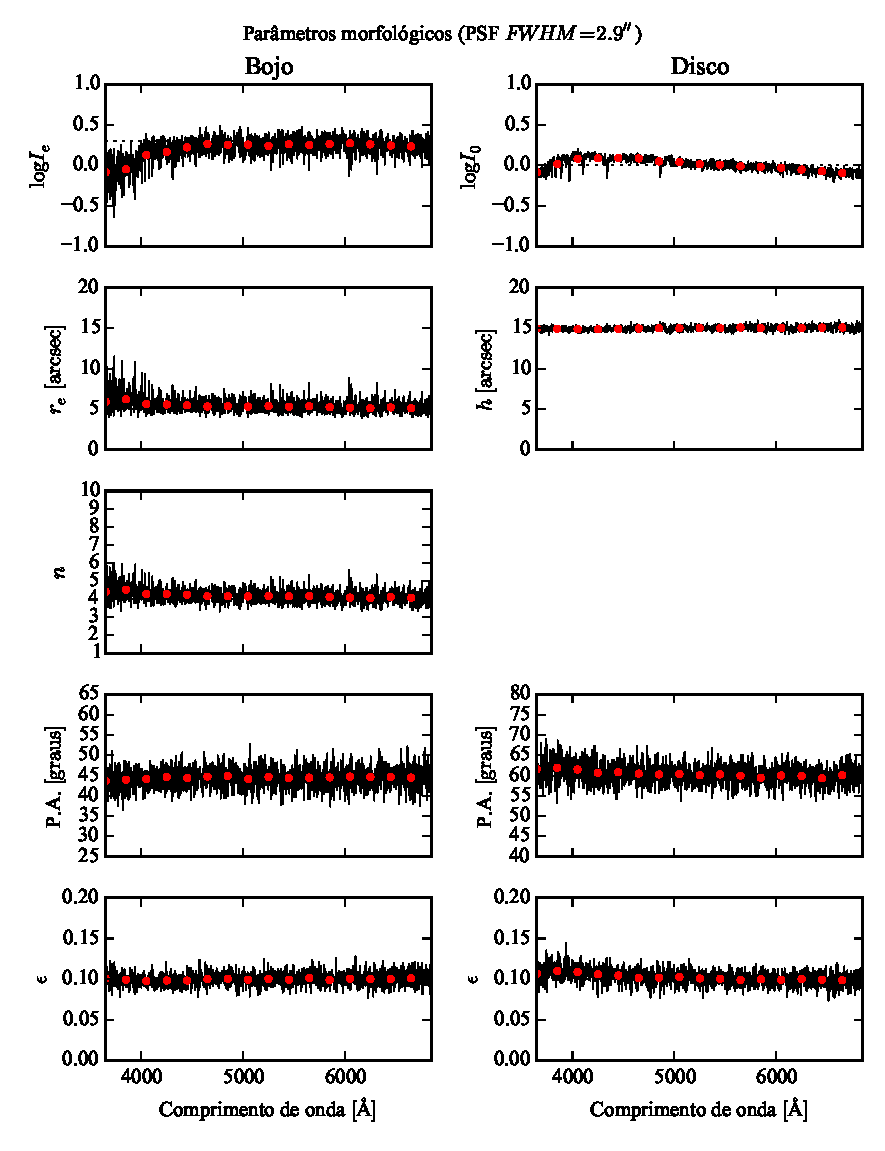
\includegraphics{figuras/simulation_fitparams}
	\caption[Parâmetros morfológicos da galáxia sintética]
	{Parâmetros morfológicos da galáxia sintética, em função do comprimento de
	onda. Pontos vermelhos: ajuste feito em caixas de $200\,\angstrom$. Linhas
	pretas: ajuste feito $\lambda$-a-$\lambda$. Linhas pontilhadas, que
	praticamente não aparecem por trás dos ajustes, são os parâmetros originais em
	$5635\,\angstrom$. Os painéis à esquerda são referentes ao bojo, e os à direita
	ao disco. Ajuste feito com uma PSF de $\mathrm{FWHM} = 2,9\,\arcs$.
	}
	\label{fig:testFitParams}
\end{figure}

os params morf ajustados sao mostrados em funcao do comprimento de onda  na fig
6.4

Os parâmetros morfológicos ajustados são mostrados em função do comprimento de
onda na Figura \ref{fig:testFitParams}. Os ajustes individuais dos parâmetros,
$\lambda$-a-$\lambda$ (linhas pretas), não se afastam muito dos parâmetros
iniciais (pontos vermelhos), e concordam bem com o modelo original (linhas
pontilhadas), praticamente escondidas atrás das linhas de ajuste na maioria dos
gráficos. Os parâmetros $r_e$ e $n$, do bojo, parecem crescer um pouco na região
abaixo de $4000\,\angstrom$, o que pode indicar uma dependência destes valores
com as características da população estelar do bojo. O ajuste do disco, por
outro lado, é praticamente constante em comprimento de onda.
os parâmetros morfológicos médios, ponderados pela verossimilhança do ajuste,
são listados na Tabela \ref{tab:testeModeloAjuste}.

\begin{table}
\begin{tabular}{ l c c l c c }
  \hline
  \multicolumn{6}{c}{\textbf{Média espectral dos modelos}} \\
  & \multicolumn{2}{c}{\textbf{Bojo}} & & \multicolumn{2}{c}{\textbf{Disco}} \\
  & \textbf{Ajuste} & \textbf{Original} & & \textbf{Ajuste} & \textbf{Original} \\
  \hline
  $r_e$ & $5,50 \pm 0.88\,\arcs$ & $5\,\arcs$ & $h$ & $14,97 \pm
  0,27\,\arcs$ & $15\,\arcs$ \\
  $n$ & $4,21 \pm 0,39$ & $4$ & & & \\
  $\mathrm{P.A.}$ & $60,4 \pm 2,4^\circ$ & $60^\circ$ & $\mathrm{P.A.}$ &
  $44,5 \pm 2,5^\circ$ & $45^\circ$ \\
  $\epsilon$ & $0,10 \pm 0,01$ & $0,1$ & $\epsilon$ & $0,10 \pm 0,01$ &
  $0,1$ \\
  \hline
\end{tabular}
\caption[Ajuste morfológico espectral -- média dos parâmetros]
{Média espectral dos parâmetros morfológicos ajustados à galáxia sintética,
ponderada pela verossimilhança dos ajustes.}
\label{tab:testeModeloAjuste}
\end{table}

Estes valores não necessariamente precisam ser iguais aos do modelo original.
Aquele foi usado para definir o modelo em $5635\,\angstrom$, e se a média
espectral se desvia dele, claramente é devido à dependência dos parâmetros
morfológicos com o comprimento de onda. Isto é, se a decomposição realmente
encontra os cubos espectrais do bojo e do disco. É preciso examinar os espectros
ajustados.

\begin{figure}
	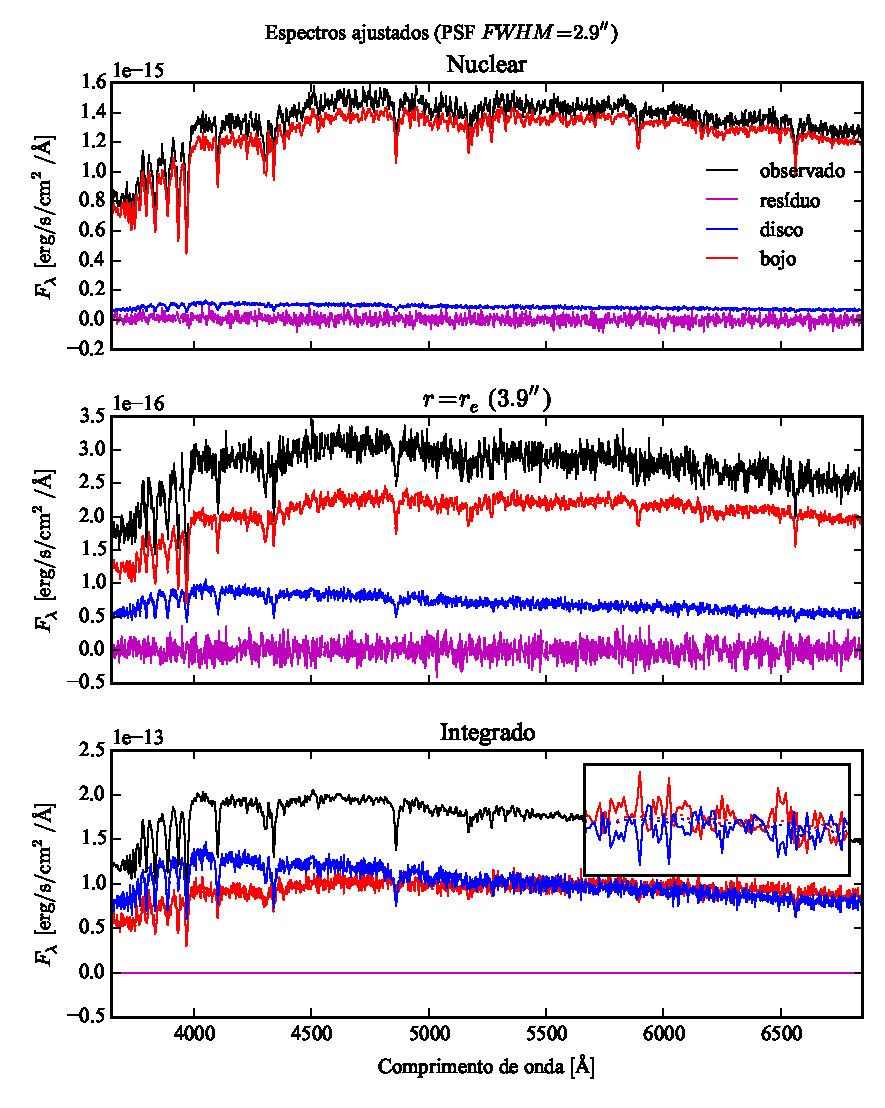
\includegraphics{figuras/simulation_spectra}
	\caption[Espectros ajustados à galáxia sintética]
	{Espectros ajustados à galáxia sintética. Em preto o espectro observado, em
	vermelho o bojo, em azul o disco, e em magenta o resíduo. Os
	espectros dos componentes originais são as linhas pontilhadas, praticamente
	cobertas pelos ajustes. Os dois painéis superiores mostram a decomposição no
	{\em spaxels} nuclear e em $r=r_e$. Os espectros integrados espacialmente são
	mostrados no painel inferior, com um {\em zoom} entre $6000$ e
	$6200\,\angstrom$ para mostrar a anti-correlação entre os ajustes de bojo e
	disco.}
	\label{fig:testFitSpectra}
\end{figure}

A Figura \ref{fig:testFitSpectra} mostra os espectros em {\em spaxels}
escolhidos (núcleo, acima, e $r=r_e$, no centro), e os espectros integrados. Os
ajustes parecem muito bons, com os espectros originais (linhas pontilhadas)
praticamente indistinguíveis dos espectros ajustados (linhas contínuas). No caso
integrado, os espectros ajustados parecem ruidosos, mas o resíduo é praticamente
nulo. Isto quer dizer que aquilo que parece ruído nos espectros é na verdade
causada por degenerescência no ajuste. As variações nas duas componentes estão
anti-correlacionadas, como se pode verificar no painel de {\em zoom} nos
espectros integrados. Esta degenerescência precisa ser estudada mais a fundo no
futuro.

\begin{figure}
	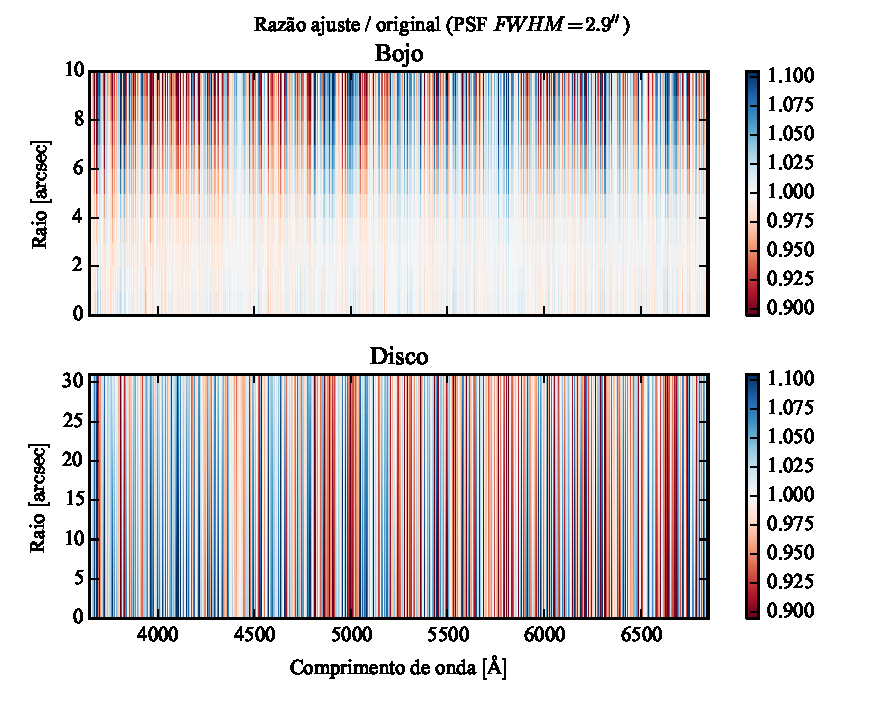
\includegraphics{figuras/simulation_error}
	\caption[Razão ajuste--original dos espectros ajustados à galáxia sintética]
	{Razão ajuste--original média dos espectros ajustados à galáxia sintética, em
	função do comprimento de onda e da distância ao centro da galáxia, tomada em
	anéis de raio constante. Valores desviando de $1$ indicam erro no ajuste.
	Acima a razão para o bojo, e abaixo para o disco. A escala radial é
	diferente nos dois casos.}
	\label{fig:testFitError}
\end{figure}

Mesmo verificando visualmente que os espectros ajustados são parecidos com os
originais, é preciso quantificar a qualidade do ajuste. Calculando a média da
razão entre o ajuste e o original, obtém-se para o bojo um valor de $1,00 \pm
0,03$. Ou seja, o ajuste tem um desvio médio de menos de $1\%$, e um desvio
padrão de $3\%$. Para o disco a razão média é $0,99 \pm 0.05$, isto é, um desvio
médio de $1\%$, e um desvio padrão de $5\%$. A ordem de magnitude destes desvios
não é nenhuma surpresa, levando em conta que foram adicionados $5\%$ de ruído
gaussiano aos dados. Mesmo assim, deve-se explorar melhor a razão
ajuste--original, para determinar se existe algum efeito sistemático nestes
desvios. A Figura \ref{fig:testFitError} mostra a razão média em anéis de raio
constante, para que seja possível fazer uma análise visual em termos de espaço e
comprimenrto de onda simultaneamente. O ajuste do bojo, mostrado no painel
superior, tem um desvio menor no centro, e vai aumentando conforme se afasta do
núcleo. Isto é esperado, já que o brilho superficial do bojo cai muito
rapidamente com o raio. O ajuste do disco, no painel inferior, parece não ter
desvios espaciais significativos.
Não há tampouco um gradiente espectral apreciável, isto é, uma cor, nas duas
componentes. Entretanto, ambas mostram o surgimento de ``linhas espectrais
artificiais'', que parecem estar anti-correlacionadas, conforme foi visto nos
espectros integrados.

Em linhas gerais, o resultado do teste é promissor. Idealmente, é necessário
testar todas as configurações possíveis de morfologia, para mapear em quais
delas a decomposição espectral é válida. Mas é preciso lembrar que o modelo
morfológico tem 7 parâmetros livres. Se cada um deles puder tomar $n$ valores
diferentes, a quantidade de modelos a serem testados é $n^7$. Com somente 4
valores por parâmetro, são mais de 16 mil modelos possíveis, o que, com cada
decomposição levando cerca de 5 minutos em um computador de 24 núcleos, leva
mais de 50 dias, sem contar o tempo necessário para análise dos resultados. Isso
sem incluir populações estelares variáveis, e diferentes PSFs (ver a Seção
seguinte). Esgotar toda a gama de modelos possíveis não é uma estratégia viável.
É preciso buscar uma abordagem mais inteligente. Também é preciso determinar se
as populações estelares das componentes modeladas, ajustadas com \starlight, são
compatíveis com as originais. Os espectros são parecidos, o que indica
populações semelhantes, mas pode haver efeitos sistemáticos. Este teste
preliminar apenas serviu para verificar que o algoritmo pode funcionar, e
justificar o seu uso em galáxias reais, do CALIFA, no próximo Capítulo.

%***************************************************************%
%                                                               %
%                   Efeitos da PSF no ajuste                    %
%                                                               %
%***************************************************************%
\section{Efeitos da PSF no ajuste}
\label{sec:test:psf}

A PSF do CALIFA foi caracterizada no Capítulo \ref{sec:psf}. Lá se verificou que
a PSF segue um perfil de Moffat com $\beta=4$ e $\mathrm{FWHM} = 2,9 \pm
0,3\,\arcs$. Os testes da Seção anterior foram feitos utilizando esta PSF, tanto
nos dados originais quanto no ajuste morfológico. Mas, dado que a FWHM da PSF
tem uma certa distribuição de valores, é justo levantar a questão: o que
acontece quando a PSF original e a utilizada na decomposição são diferentes? Em
outras palavras, como se comporta a decomposição morfológica espectral quando
não temos um conhecimento perfeito da PSF?

Para tentar compreender o efeito de uma PSF inadequada aos dados na
decomposição, o teste foi refeito, porém com a galáxia original sintética
convoluída com PSFs de $\mathrm{FWHM} = 2,6\,\arcs$ e $\mathrm{FWHM} =
3,3\,\arcs$. Com isto tem-se valores próximos aos limites dados pela incerteza
na medida da PSF do CALIFA. A mesma PSF de $\mathrm{FWHM} = 2,9\,\arcs$ foi
utilizada na decomposição morfológica espectral. No caso da galáxia sintética
com a PSF de $2,6\,\arcs$, o ajuste está sobre-estimando o valor da FWHM real,
enquanto no caso da galáxia com $3,3\,\arcs$ a FWHM é subestimada.

\begin{figure}
	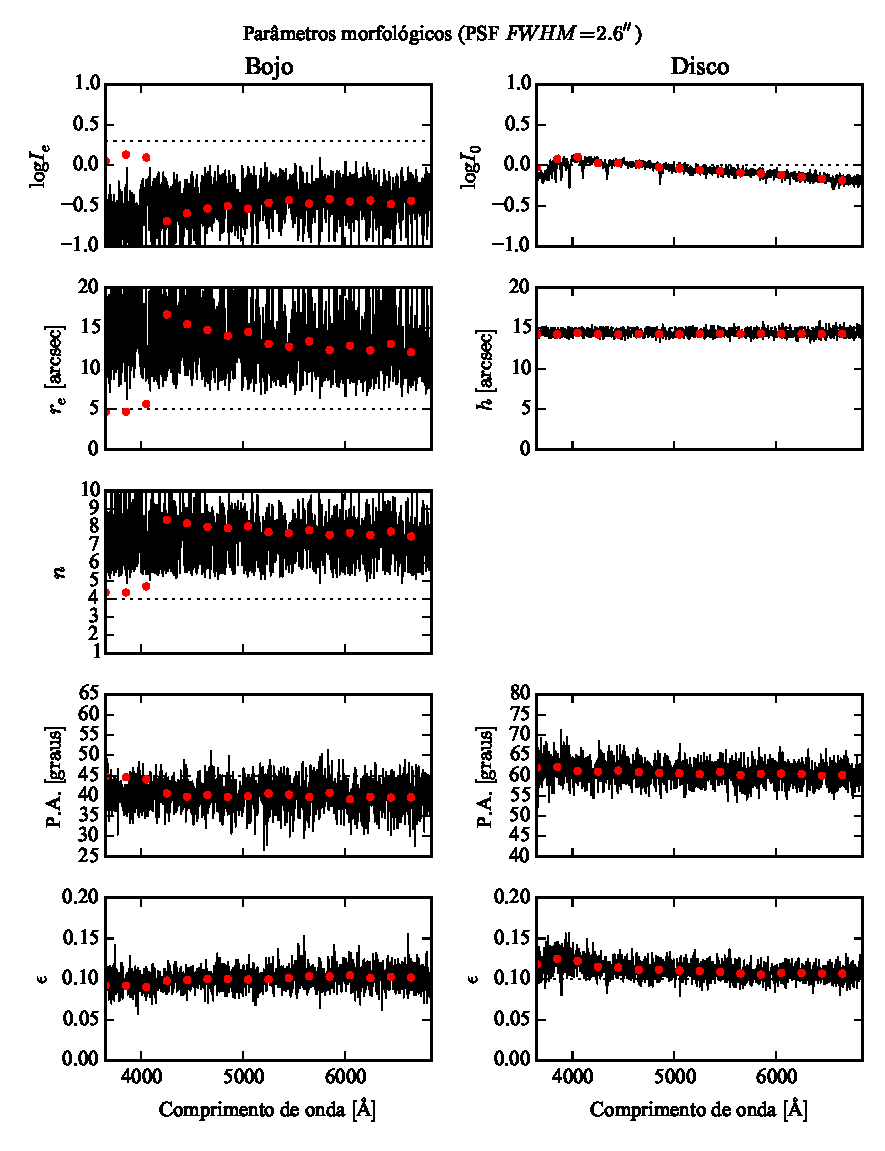
\includegraphics{figuras/simulation_fitparams_psf26}
	\caption[Parâmetros morfológicos (teste com PSF $\mathrm{FWHM} = 2,6\,\arcs$)]
	{Parâmetros morfológicos da galáxia sintética, em função do comprimento de
	onda. Ajuste feito com uma PSF de $\mathrm{FWHM} = 2,9\,\arcs$ sobre
	dados com $\mathrm{FWHM} = 2,6\,\arcs$. Ver legenda da Figura
	\ref{fig:testFitParams}.}
	\label{fig:testFitParams26}
\end{figure}

\begin{figure}
	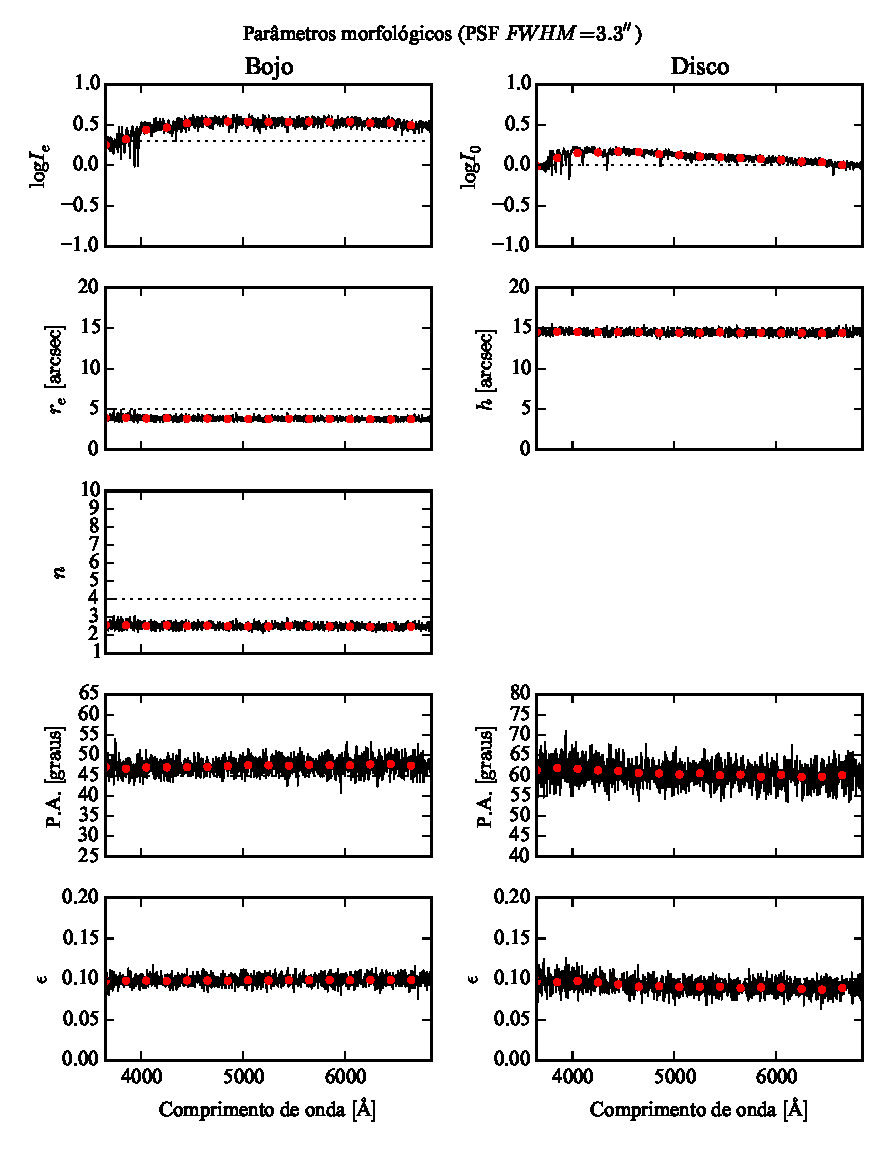
\includegraphics{figuras/simulation_fitparams_psf33}
	\caption[Parâmetros morfológicos (teste com PSF $\mathrm{FWHM} =
	3,3\,\arcs$)] {Parâmetros morfológicos da galáxia sintética, em função do comprimento de
	onda. Ajuste feito com uma PSF de $\mathrm{FWHM} = 2,9\,\arcs$ sobre
	dados com $\mathrm{FWHM} = 3,3\,\arcs$. Ver legenda da Figura
	\ref{fig:testFitParams}.}
	\label{fig:testFitParams33}
\end{figure}

As Figuras \ref{fig:testFitParams26} e \ref{fig:testFitParams33} mostram os
parâmetros morfológicos obtidos para os dois casos. Pode-se ver que os
parâmetros obtidos para o disco são muito próximos dos parâmetros do teste
anterior. Não é de se estranhar, pois o disco é muito suave e não tem estruturas
na escala de tamanho da PSF. O bojo, por outro lado, é muito afetado pela má
escolha da PSF. {\em Sobre-estimar} a FWHM da PSF ($2,9\,\arcs > 2,6\,\arcs$)
faz os valores de $r_e$ e $n$ aumentarem muito, de $5\,\arcs$ e $4$ para cerca
de $13\,\arcs$ e $7$, respectivamente. Também aumenta a dispersão nos dois
parâmetros, provavelmente causado por degenerescência no ajuste. Com a FWHM {\em
subestimada} ($2,9\,\arcs < 3,3\,\arcs$), os valores destes parâmetros diminui,
com $r_e \sim 4\,\arcs$ e $n \sim 2,5$. O disco muda pouco, como no outro caso.
Os parâmetros médios das duas decomposições são listados na Tabela
\ref{tab:testeAjustePSF}.

\begin{table}
\begin{tabular}{ l c c  l c c }
  \hline
  \multicolumn{6}{c}{\textbf{Média espectral dos modelos (PSF diferente)}} \\
  & \multicolumn{2}{c}{\textbf{Bojo}} & & \multicolumn{2}{c}{\textbf{Disco}} \\
  & $\mathrm{FWHM} = 2,6\,\arcs$ & $\mathrm{FWHM} = 3,3\,\arcs$ & &
  $\mathrm{FWHM} = 2,6\,\arcs$ & $\mathrm{FWHM} = 3,3\,\arcs$ \\
  \hline
  $r_e$ & $13,64 \pm 5.22\,\arcs$ & $3,83 \pm 0,22\,\arcs$ & $h$ & $14,40
  \pm 0.38\,\arcs$ & $14,47 \pm 0,27\,\arcs$ \\
  $n$ & $7,38 \pm 1,25$ & $2,51 \pm 0,13$ & & & \\
  $\mathrm{P.A.}$ & $60,7 \pm 2,6^\circ$ & $60,5 \pm
  2,6^\circ$ & $\mathrm{P.A.}$ & $40,2 \pm 3.6^\circ$ & $47.4 \pm
  1.7^\circ$ \\
  $\epsilon$ & $0,11 \pm 0,01$ & $0,09 \pm 0,01$ & $\epsilon$ & $0,10 \pm
  0,01$ & $0,099 \pm 0,01$ \\
  \hline
\end{tabular}
\caption[Parâmetros do ajuste morfológico espectral com PSF diferente]
{Média espectral dos parâmetros morfológicos ajustados à galáxia sintética,
ponderada pela verossimilhança dos ajustes, com a PSF do ajuste ($\mathrm{FWHM}
= 2,9\,\arcs$) diferente da PSF dos dados.}
\label{tab:testeAjustePSF}
\end{table}

\begin{figure}
	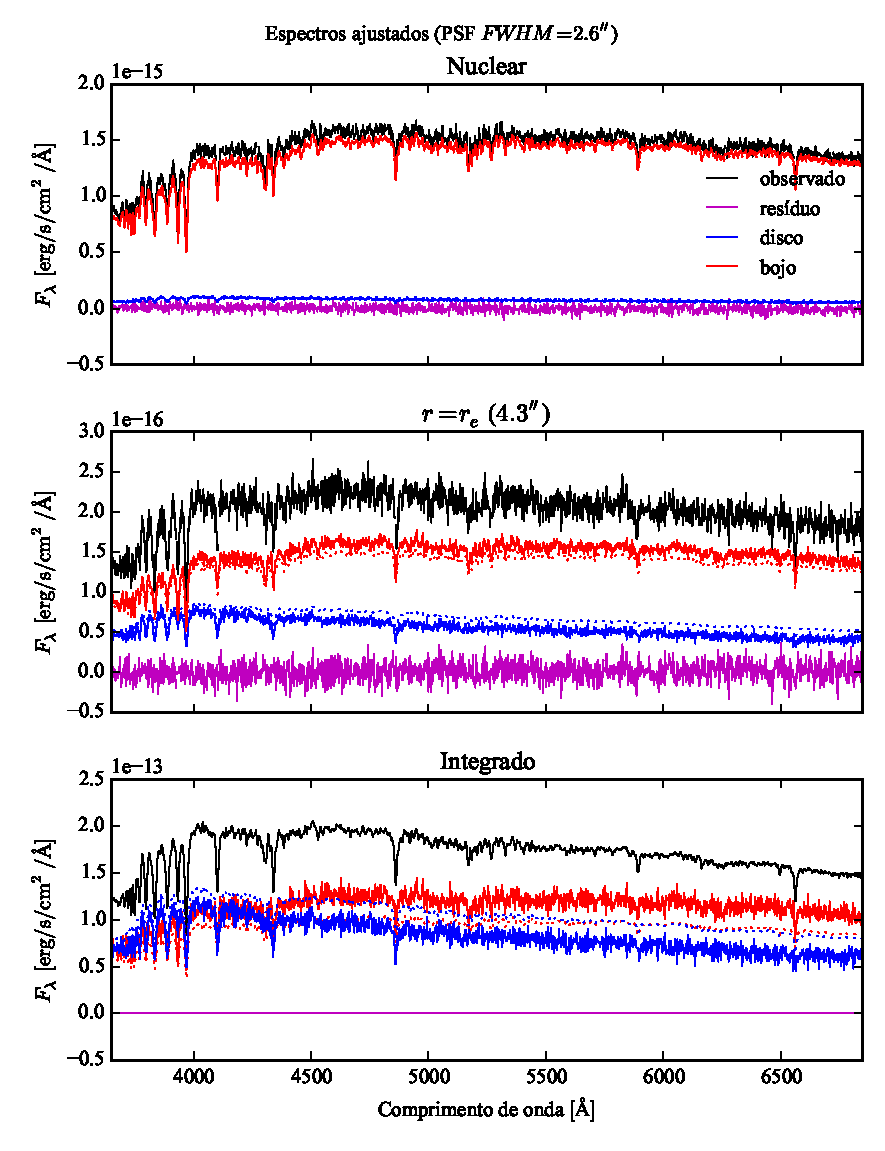
\includegraphics{figuras/simulation_spectra_psf26}
	\caption[Espectros ajustados (teste com PSF $\mathrm{FWHM} = 2,6\,\arcs$)]
	{Espectros ajustados à galáxia sintética. Ajuste feito com uma PSF de
	$\mathrm{FWHM} = 2,9\,\arcs$ sobre dados com $\mathrm{FWHM} = 2,6\,\arcs$. Ver
	legenda da Figura \ref{fig:testFitSpectra}.}
	\label{fig:testFitSpectra26}
\end{figure}

\begin{figure}
	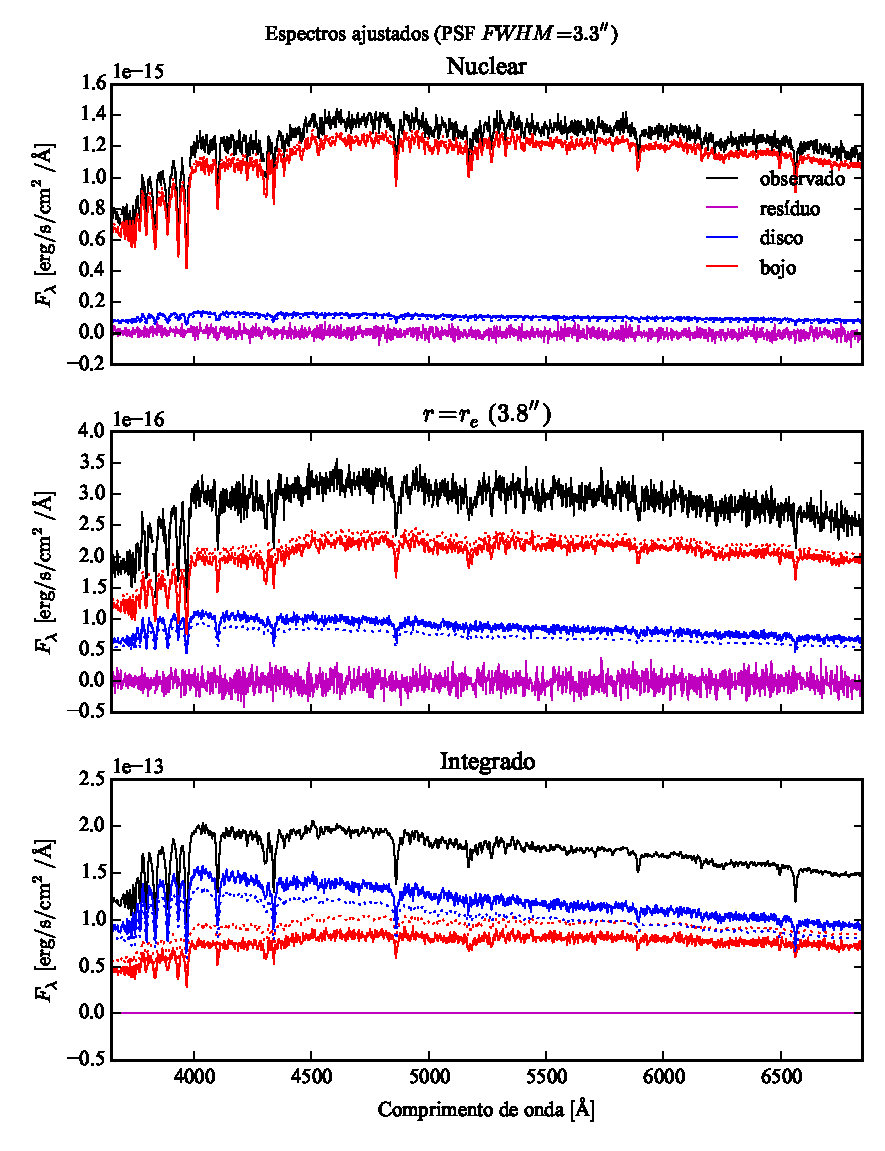
\includegraphics{figuras/simulation_spectra_psf33}
	\caption[Espectros ajustados (teste com PSF $\mathrm{FWHM} = 3,3\,\arcs$)]
	{Espectros ajustados à galáxia sintética. Ajuste feito com uma PSF de
	$\mathrm{FWHM} = 2,9\,\arcs$ sobre dados com $\mathrm{FWHM} = 3,3\,\arcs$. Ver
	legenda da Figura \ref{fig:testFitSpectra}.} \label{fig:testFitSpectra33}
\end{figure}

A dispersão nos parâmetros do bojo, no caso sobre-estimado, parece um problema
em potencial. Percebe-se, porém, que a dispersão nos parâmetros não se reflete
tanto nos espectros, como mostra a Figura \ref{fig:testFitSpectra26}. Os
espectros são parecidos com os originais, com diferenças sistemáticas e um
``ruído'' maior do que o ajuste com a PSF correta. No caso subestimado, os
espectros parecem melhor ajustados (Figura \ref{fig:testFitSpectra33}), mas
também com com diferenças sistemáticas.

\begin{figure}
	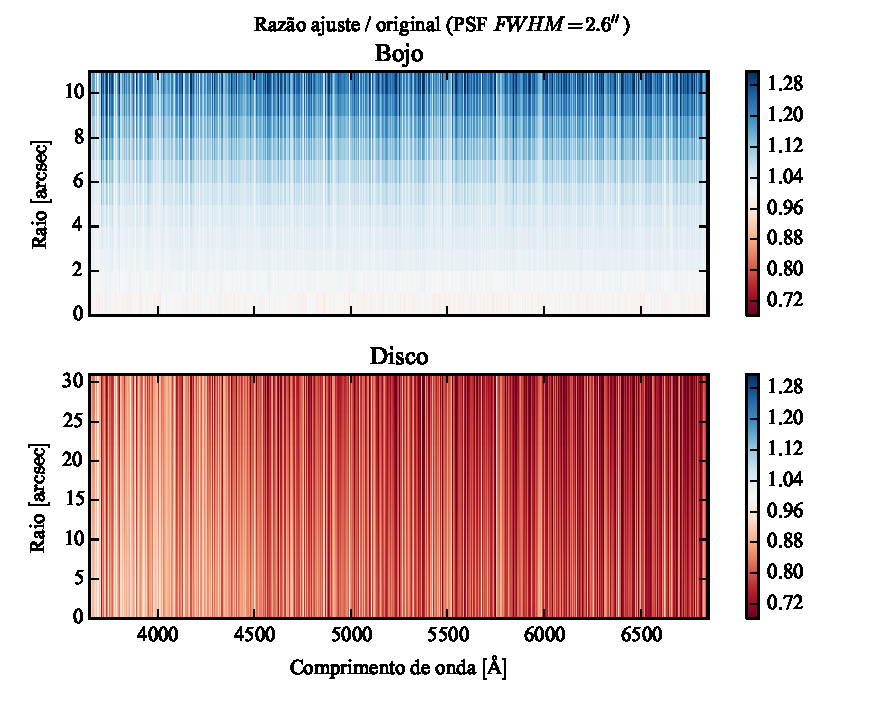
\includegraphics{figuras/simulation_error_psf26}
	\caption[Razão ajuste--original (teste com PSF $\mathrm{FWHM} = 2,6\,\arcs$)]
	{Razão ajuste--original média dos espectros ajustados à galáxia sintética.
	Ajuste feito com uma PSF de $\mathrm{FWHM} = 2,9\,\arcs$ sobre
	dados com $\mathrm{FWHM} = 2,6\,\arcs$. Ver legenda da Figura
	\ref{fig:testFitError}.}
	\label{fig:testFitError26}
\end{figure}

\begin{figure}
	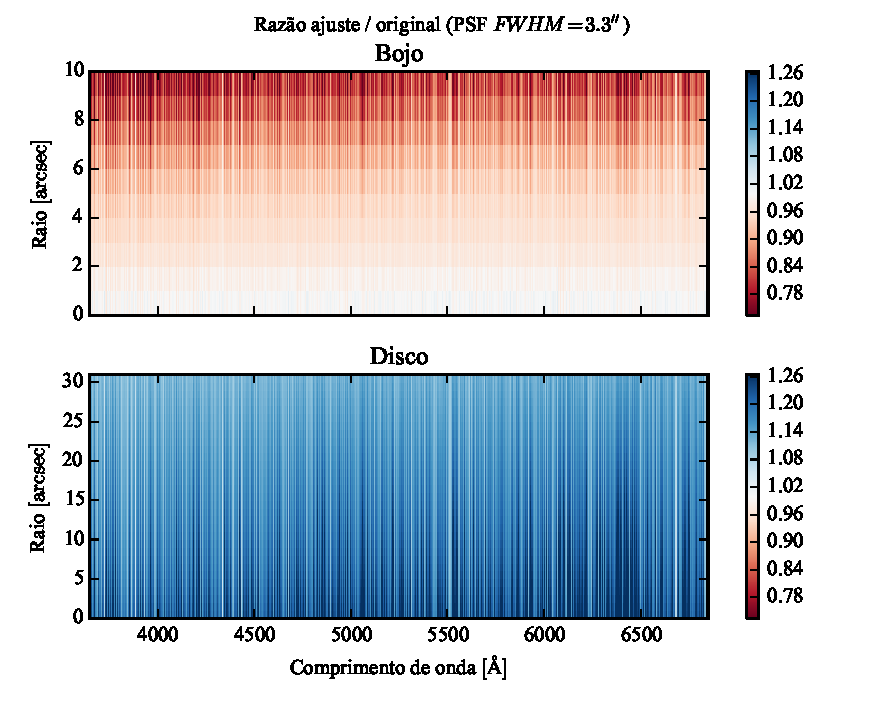
\includegraphics{figuras/simulation_error_psf33}
	\caption[Razão ajuste--original (teste com PSF $\mathrm{FWHM} = 3,3\,\arcs$)]
	{Razão ajuste--original média dos espectros ajustados à galáxia sintética.
	Ajuste feito com uma PSF de $\mathrm{FWHM} = 2,9\,\arcs$ sobre
	dados com $\mathrm{FWHM} = 3,3\,\arcs$. Ver legenda da Figura
	\ref{fig:testFitError}.}
	\label{fig:testFitError33}
\end{figure}

Fazendo a razão ajuste--original (Figura \ref{fig:testFitError26}), percebe-se
que espectro ajustado do bojo torna-se maior do que o original conforme se
afasta do centro, enquanto o disco apresenta um gradiente espectral, ficando
mais azul, quando se sobre-estima a FWHM. As ``linhas espectrais artificiais''
neste caso são bem pronunciadas. A razão média para o bojo é de $1,06 \pm 0,06$,
e para o disco de $0,77 \pm 0,08$. Quando se subestima a FWHM (Figura
\ref{fig:testFitError33}), o espectro ajustado do bojo é mais fraco e do que o
original, e diminui com o raio. O disco não parece ter gradiente radial, e, em
ambos os casos, não há um gradiente espectral perceptível, com ``linhas
espectrais artificiais'' menos intensas do que no outro caso. A razão média
neste caso é $0,94 \pm 0,05$ para o bojo e $1,13 \pm 0.04$ para o disco.

Ao se utilizar, na decomposição morfológica, uma PSF com FWHM maior do que a
real (superestimando), é impossível criar um modelo com um bojo tão concentrado
quanto o observado. O que acontece então é que o algoritmo chega aos modelos
mais próximos, que não representam exatamente a galáxia. O mesmo não ocorre
quando se utiliza uma FWHM menor. Neste caso, basta fazer um bojo menos
concentrado ($r_e$ e/ou $n$ menor). Pelo teste, este caso é mais estável, isto
é, possui menos degenerescência.

Assim, pode-se ficar tentado a utilizar a PSF com FWHM menor na decomposição
morfológica espectral das as galáxias do CALIFA, a fim de evitar os caso onde se
superestima a PSF. Utilizando uma PSF menor pode-se ter a ilusão de obter o
resultado da decomposição para mais galáxias. Entretanto, deve-se lembrar que o
ajuste é significativamente melhor quando se usa a PSF correta, e apresentando
menos artefatos na dependência dos parâmetros morfológicos com o comprimento de
onda. Com uma PSF menor, conforme visto na distribuição da Figura
\ref{fig:PSFCalib}, a probabilidade é muito pequena de que algumas das galáxias
tenham sido observadas com aquela PSF. Como a decomposição morfológica espectral
é um método experimental, o melhor é utilizar a PSF mais frequente da
distribuição, de $\mathrm{FWHM} = 2,9\,\arcs$, e selecionar somente as galáxias
onde a decomposição parece ter um menor espalhamento no ajuste dos parâmetros em
função do comprimento de onda. A decomposição é, provavelmente, mais confiável
nestes casos.

%% End of this chapter
